\documentclass{beamer}
\usepackage{graphicx}
\usepackage{hyperref}
\usepackage{mathtools}
\usepackage{tikz}

\title{Simulation of two interacting squirmers}
\author{Robin Roth and Justine Ehret}
\institute{Supervised by: Van Landeghem Céline, Giraldi Laetitia}

\begin{document}
\begin{frame}
    \titlepage
\end{frame}

\begin{frame}
    \tableofcontents
\end{frame}

\section{What is a squirmer ?}
\begin{frame}{What is a squirmer ?}
    \begin{columns}[T]
        \begin{column}{0.5\textwidth}
            \begin{itemize}
                \item Introduced by James Lighthill in 1952 \cite{Wikipedia}
                \item Extended by John Blake in 1971 \cite{Wikipedia}
                \item Model for a spherical microswimmer
                \item Cannot model cilia so we impose boundary conditions
                \begin{itemize}
                    \item Tangential time-independant velocity at the boundary, propelling the squirmers.
                    \item In particullar, we fix the type $\beta$ and the speed $B1$.
                \end{itemize}
            \end{itemize}
        \end{column}
        \begin{column}{0.5\textwidth}
            \centering
            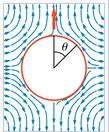
\includegraphics[width=\textwidth]{../images/squirmer.png}
            \cite{Wikipedia}
        \end{column}
    \end{columns}
\end{frame}

\section{Objectives}
\begin{frame}{Objectives}
    \begin{itemize}
        \item Understand the "Squirmers" model
        \item Study the dynamics between two squirmers
        \begin{itemize}
            \item Study the interactions between two squirmers \cite{Brumley}\cite{Lauga}
            \item Rewrite the existing code from Matlab to Python
            \item Develop code to calculate the missing torques
        \end{itemize}
        \item Numerical Experiments
        \begin{itemize}
            \item Verify if our results align with previous studies\cite{Brumley}\cite{Lauga}\cite{Stark}
            \item Verify if changing the value of $\beta$ and the initial distance affect the behavior
        \end{itemize}
    \end{itemize}
\end{frame}

\section{Roadmap}
\begin{frame}{Roadmap}
    \begin{center}
        \href{https://github.com/orgs/master-csmi/projects/23/views/2}{Roadmap}
        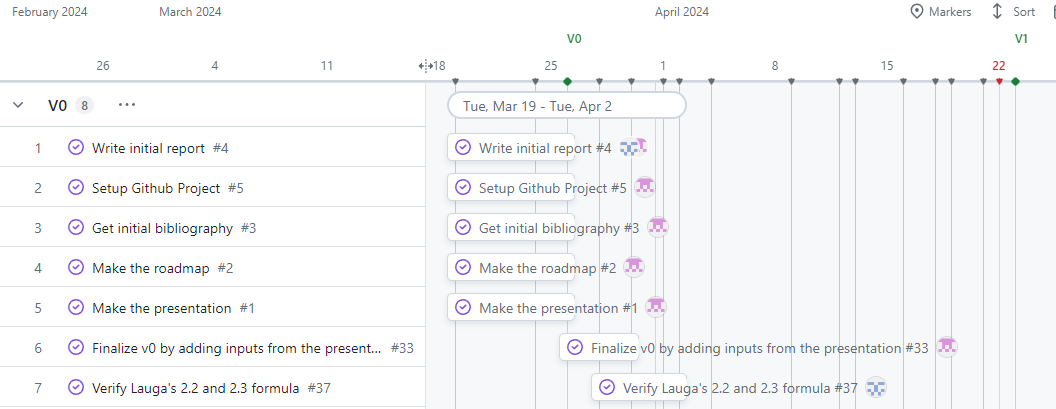
\includegraphics[width=0.9\textwidth]{../images/roadmapV0_1.png}
        \vspace{1em}
        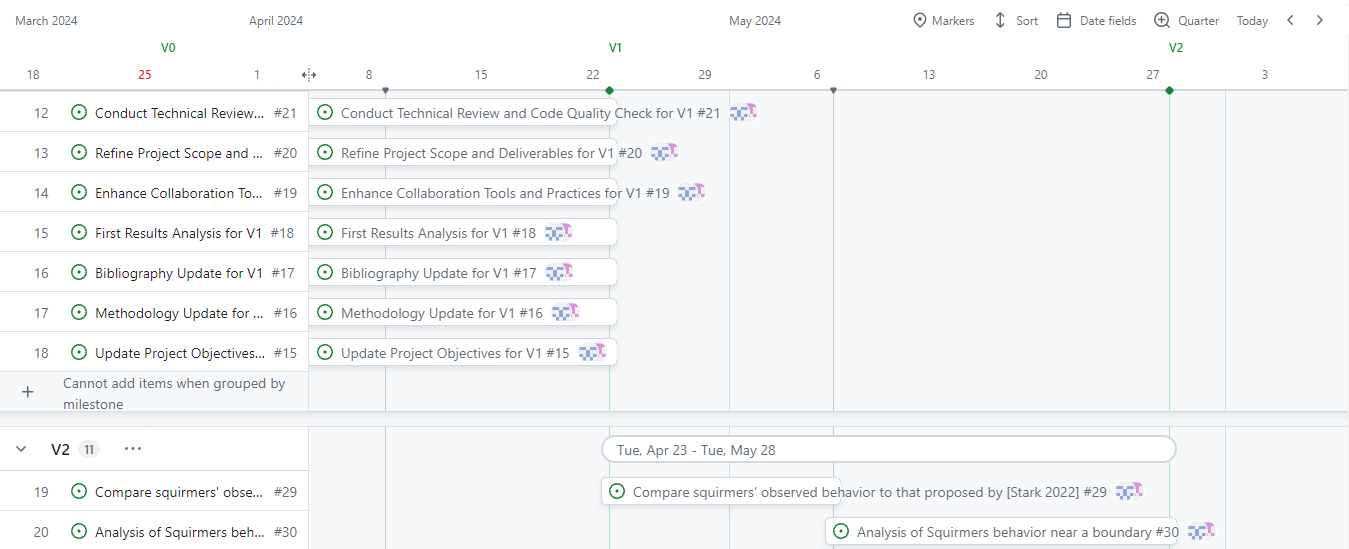
\includegraphics[width=0.9\textwidth]{../images/roadmapV0_2.png}
    \end{center}
\end{frame}
\begin{frame}{Roadmap}
    \begin{center}
        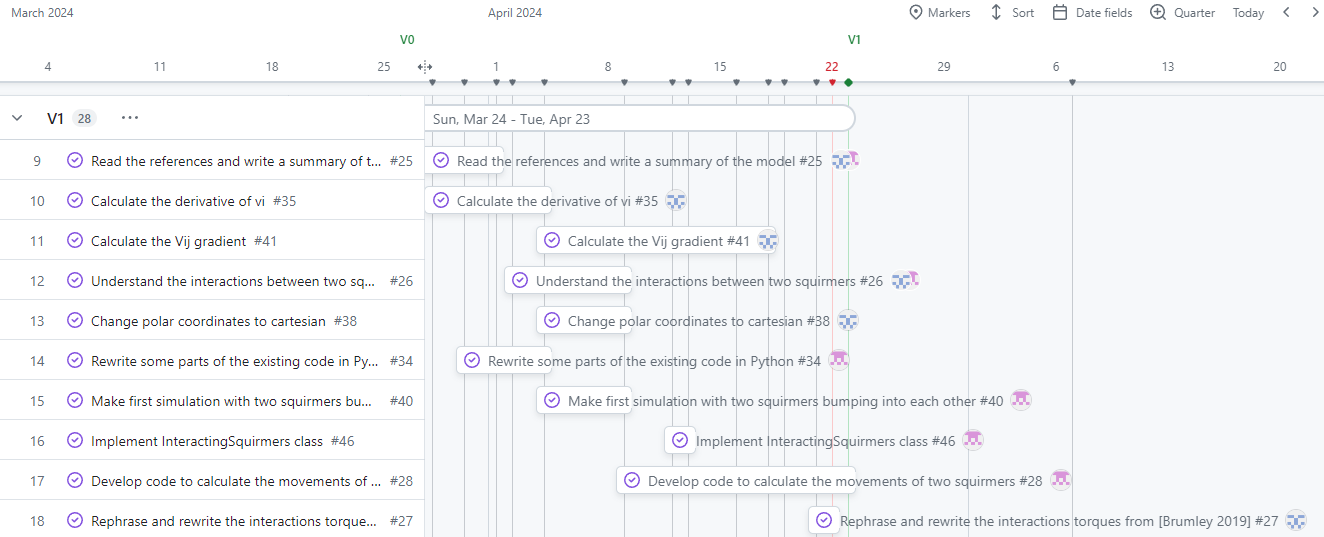
\includegraphics[width=0.9\textwidth]{../images/roadmapV1_1.png}
        \vspace{1em}
        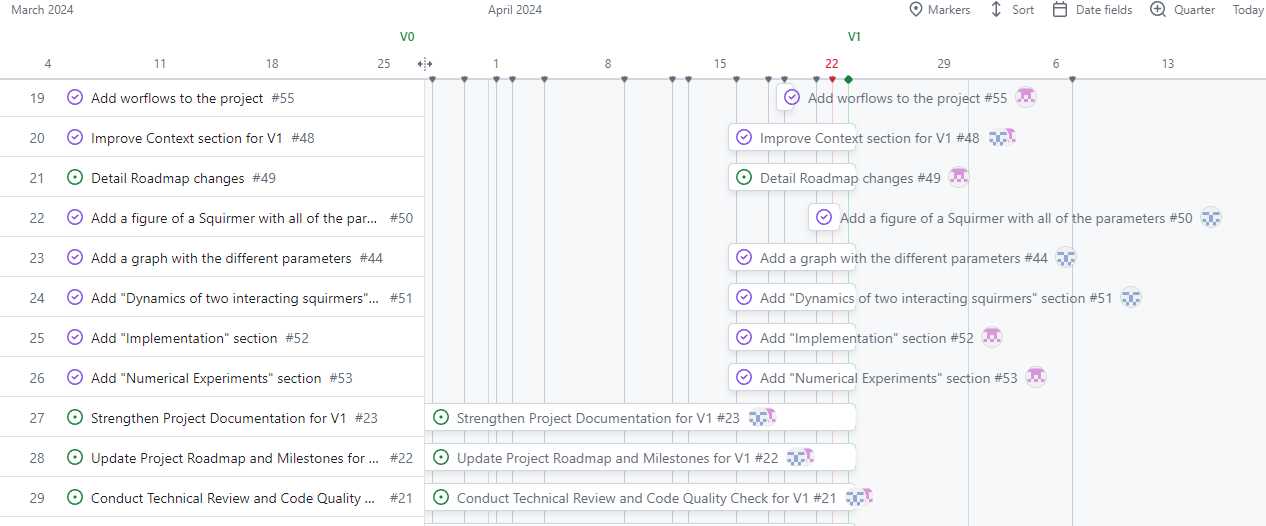
\includegraphics[width=0.9\textwidth]{../images/roadmapV1_2.png}
    \end{center}
\end{frame}

\begin{frame}{Roadmap}
    \begin{center}
        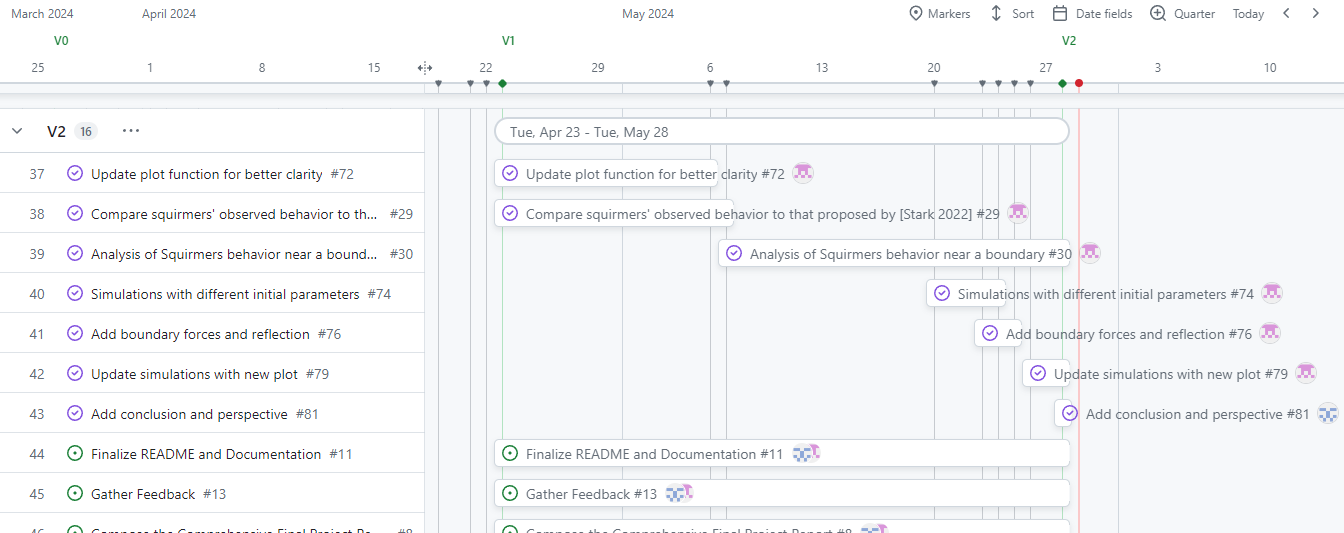
\includegraphics[width=0.9\textwidth]{../images/roadmapV2.png}
    \end{center}
\end{frame}

\section{Squirmer model}
\begin{frame}{Squirmer model}
    \begin{center}
        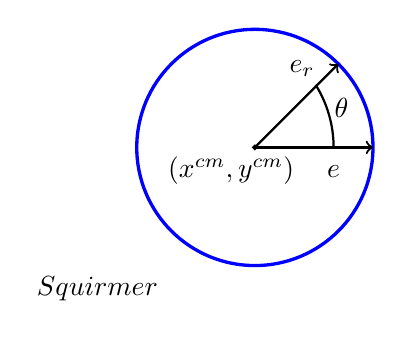
\begin{tikzpicture}
        
        \draw[color=blue, very thick](2.5,2.5) circle (1.5);
        
        \draw[color=black, very thick](2.5,2.5) circle (0.01);
        
        \node  at (2.5-0.3,2.5-0.3) {{$(x^{cm},y^{cm})$}};
        
        \node  at (0.5,0.7) {{$Squirmer$}};
        
        \draw[thick, ->] (2.5,2.5) -- (4,2.5);
        \node  at (3.5,2.2) {{$e$}};
     
        \pgfmathsetmacro{\xcoord}{2.5 + 1.5*cos(45)}
         \pgfmathsetmacro{\ycoord}{2.5 + 1.5*sin(45)}
         \draw[thick, ->] (2.5,2.5) -- (\xcoord,\ycoord);
        \node  at (3.1,3.5) {{$e_r$}}; 
        \draw[thick, -] (3.5,2.5) arc[start angle=0, end angle=32, radius=1.5];
        \node at (3.6,3) {${\theta}$}; 
        
           
        \end{tikzpicture}
        \end{center}
    \begin{itemize}
        \item The velocity $u$ in polar coordinates \cite{Lauga} : \begin{align*}
       \left\{\begin{array}{rcl}
          u_r(R,\theta) &=& 0 \\
          u_\theta(R,\theta) &=& B_1(\mathrm{sin}(\theta) + \beta \mathrm{sin}(\theta)\mathrm{cos}(\theta)),
       \end{array}\right.\;
        \end{align*} with $\beta=\frac{B_2}{B_1}$ :
    $\left\{
        \begin{array}{ll}
            \beta = 0 : \text{neutral swimmer}  \\
            \beta < 0 : \mathrm{pusher} \\
            \beta > 0 : \mathrm{puller} \\
        \end{array}
    \right.$
        \item In  cartesian coordinates :
        $u_r = B_1(1+\beta (e\cdot e_r)) [(e\cdot e_r)e_r - e]$
    \end{itemize}
\end{frame}
    
\section{Dynamics of two interacting squirmers}
\subsection{The evolution of the mass center $R_i$}    
\begin{frame}{Dynamics of two interacting squirmers}
        \framesubtitle{The evolution of the mass center $R_i$}
        The evolution of the mass center $R_i$ = $(X_i, Y_i)$ of one squirmer $i$ in presence of 
    another squirmer $j$ and rigid boundaries, is given by :
    \begin{center}
    $\boxed{\frac{dR_i}{dt}$ = $v_0 p_i -  \nabla_{R_{ij}} V_{ij} - \nabla_{R_i} V_i + F^{hydro}}$
    \end{center}
    We have : \begin{itemize}
        \item $v_0$ the particle swimming velocity,
        \item $p_i$ = $(\mathrm{cos}(\theta),\mathrm{sin}(\theta))$ orientation,
        \item $F^{hydro}$ the lubrification forces given by Brumley\cite{Brumley},
        \item $V_{ij}$ and $V_i$, Weeks-Chandler-Andersen potential : repulsive steric force avoiding the overlapping of two squirmers or of one squirmer and a rigid boundary. The force is activated when the distance between two surfaces is small.
    \end{itemize}
\end{frame}
    
\begin{frame}{Dynamics of two interacting squirmers}
    \framesubtitle{The evolution of the mass center $R_i$}
    \begin{center}
        \(\boxed{\frac{dR_i}{dt} = v_0 p_i -  \nabla_{R_{ij}} V_{ij} - \nabla_{R_i} V_i + F^{hydro}}\)
    \end{center}
    We have: 
    \begin{itemize}
        \item \(\nabla_{R_{ij}} V_{ij} = 
        \begin{pmatrix}
            \frac{-3 E_s}{r} \frac{D_x}{\sqrt{R_{ij}}}\left[ \frac{2(2r)^{13}}{(R_{ij})^{13}} - \frac{(2r)^7}{(R_{ij})^7} \right] \\
            \frac{-3 E_s}{r} \frac{D_y}{\sqrt{R_{ij}}}\left[ \frac{2(2r)^{13}}{(R_{ij})^{13}} - \frac{(2r)^7}{(R_{ij})^7} \right]
        \end{pmatrix}\)
        \item \(\nabla_{R_i} V_i = 
        \begin{pmatrix}
            -6 \frac{E_s (X-X_{box})}{r \lvert R - R_i \rvert } \left[ 2 \left( \frac{r}{\lvert R-R_i\rvert} \right)^{13} - \left( \frac{r}{\lvert R-R_i\rvert}\right)^7 \right] \\
            -6 \frac{E_s (Y-Y_{box})}{r \lvert R - R_i \rvert } \left[ 2 \left( \frac{r}{\lvert R-R_i\rvert} \right)^{13} - \left( \frac{r}{\lvert R-R_i\rvert}\right)^7 \right]
        \end{pmatrix}\)
    \end{itemize}
    \end{frame}
    
    \begin{frame}{Dynamics of two interacting squirmers}
        \begin{center}
       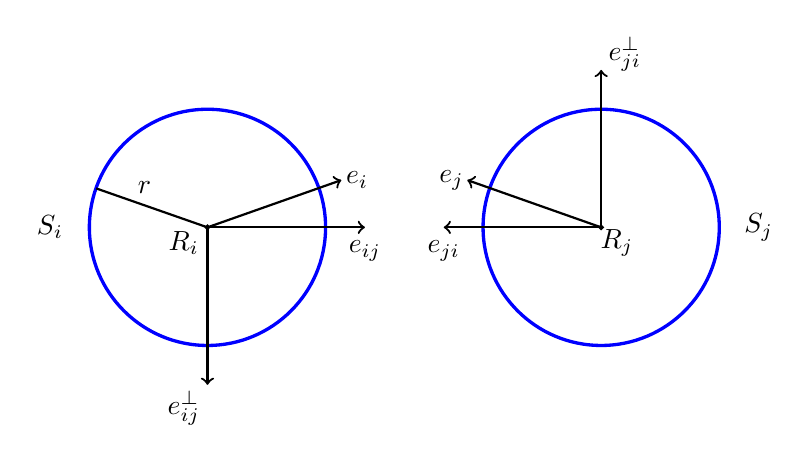
\begin{tikzpicture}
       
       \draw[color=blue, very thick](5,5) circle (1.5);
       \draw[color=blue, very thick](0,5) circle (1.5);
       
       \draw[color=black, very thick](0,5) circle (0.01);
       \draw[color=black, very thick](5,5) circle (0.01);
       
       \node  at (-0.3,5-0.2) {{$R_i$}};
       \node  at (5+0.2,5-0.2) {{$R_j$}};
       
       \node  at (-2,5) {{$S_i$}};
       \node  at (7,5) {{$S_j$}};
       
       \draw[thick, ->] (0,5) -- (1.7,5+0.6);
       \draw[thick, ->] (5,5) -- (5-1.7,5+0.6);
       
       \node  at (1.9,5+0.6) {{$e_i$}};
       \node  at (5-1.9,5+0.6) {{$e_j$}};
       
       \draw[thick] (0,5) -- ({-cos(45)*2}, {5+0.7*sin(45)});
       \node  at (-0.8,5+0.5) {{$r$}};
       
       \draw[thick, ->] (0,5) -- (2,5);
       \draw[thick, ->] (5,5) -- (3,5);
       
       \node  at (2,5-0.3) {{$e_{ij}$}};
       \node  at (3,5-0.3) {{$e_{ji}$}};
       
       \draw[thick, ->] (0,5) -- (0,3);
       \node  at (-0.3,3-0.3) {$e^{\perp}_{ij}$};
       
       
       \draw[thick, ->] (5,5) -- (5,7);
       \node  at (5+0.3,7+0.2) {$e^{\perp}_{ji}$};
       
       \end{tikzpicture}
       \end{center}
       The figure shows the different vectors involved in the computations which will follow.
        
\end{frame}
    
    \begin{frame}{Dynamics of two interacting squirmers}
        \begin{itemize}
            \item The tangential lubrification forces acting on the two spheres : \begin{equation*}
    \footnotesize
    \boxed{
        \begin{aligned}
        F_z^{S_i} = & -9 \mu \pi r \frac{\lambda ^2}{(\lambda +1)^2} \left[ -B_1 \sin(\theta)\cos(\theta) - \frac{1}{2} B_1  \cos(\theta) (e_i \cdot e^{\perp}_{ij})^2 \right. \\
        & \left. -B_2 \cos^2(\theta) - \frac{1}{2} B_2 (e_i \cdot e^{\perp}_{ij})^2 (e_i \cdot e^{\perp}_{ij})^2 \right] (\ln \epsilon + O(1))
        \end{aligned}
    }
    \end{equation*}
        \item The normal forces acting on the two spheres :
        \begin{equation*}
        \boxed{F_x^{S_i} = -\frac{4}{5} \mu \pi r \frac{\lambda(\lambda +4)}{(\lambda +1)^2} \left[ -B_1\mathrm{sin}(\theta) -B_2\mathrm{cos}(\theta)\mathrm{sin}(\theta)\right] (ln \epsilon + O(1))}
    \end{equation*}
        \end{itemize}
    
\end{frame}
    
\subsection{The evolution of the orientation $\theta _i$}
\begin{frame}{Dynamics of two interacting squirmers}
        \framesubtitle{The evolution of the orientation $\theta _i$}
    The evolution of the rotation of one squirmer is given by : 
    $$
    \frac{d \theta_i}{dt} = \sum \Gamma_{ij->i} + \sum \Gamma_{ji->i} +  \Gamma_{i}^W.
    $$ 
    $\Gamma_{ij->k}$ is the torque exerted on the $k^\mathrm{th}$ particle by the flow associated to the $i^\mathrm{th}$ particle, but perturbed by the presence of the $j^\mathrm{th}$ particle.
    
    \begin{itemize}
        \item The torques acting on the squirmer $i$ :
        \begin{equation*}
        \footnotesize
        \boxed{T_y^{S_i} = \frac{16 \lambda}{5(\lambda +1)} \mu \pi r^2 e_i.e^{\perp}_{ij}\left[-B_1\mathrm{sin}(\theta) -B_2\mathrm{cos}(\theta)\mathrm{sin}(\theta) \right] (ln \epsilon + O(1))}
    \end{equation*}
        \item The torques acting on the squirmer $j$ :
        \begin{equation*}
        \footnotesize
        \boxed{T_y^{S_j} = \frac{4 \lambda^2}{5(\lambda +1)} \mu \pi r^2 e_i.e^{\perp}_{ij}\left[-B_1\mathrm{sin}(\theta) -B_2\mathrm{cos}(\theta)\mathrm{sin}(\theta) \right] (ln \epsilon + O(1))}
    \end{equation*}
    \end{itemize}
        
\end{frame}

\section{Implementation in Python}
\begin{frame}{Implementation in Python}
    
% \end{frame}

\begin{frame}{Numerical Experiments}
    \begin{center}
        First simulation
        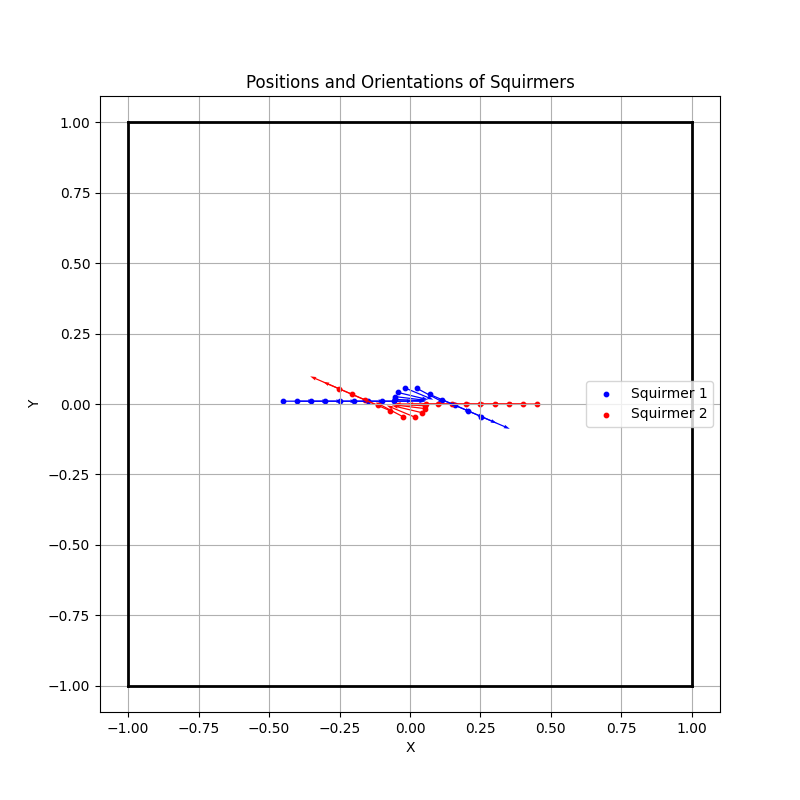
\includegraphics[width=0.8\textwidth]{../../graphs/squirmers_colliding.png}
    \end{center}
\end{frame}

\section{Numerical Experiments}
\begin{frame}{Numerical Experiments}
    \begin{center}
        Results from previous study \cite{Stark}
        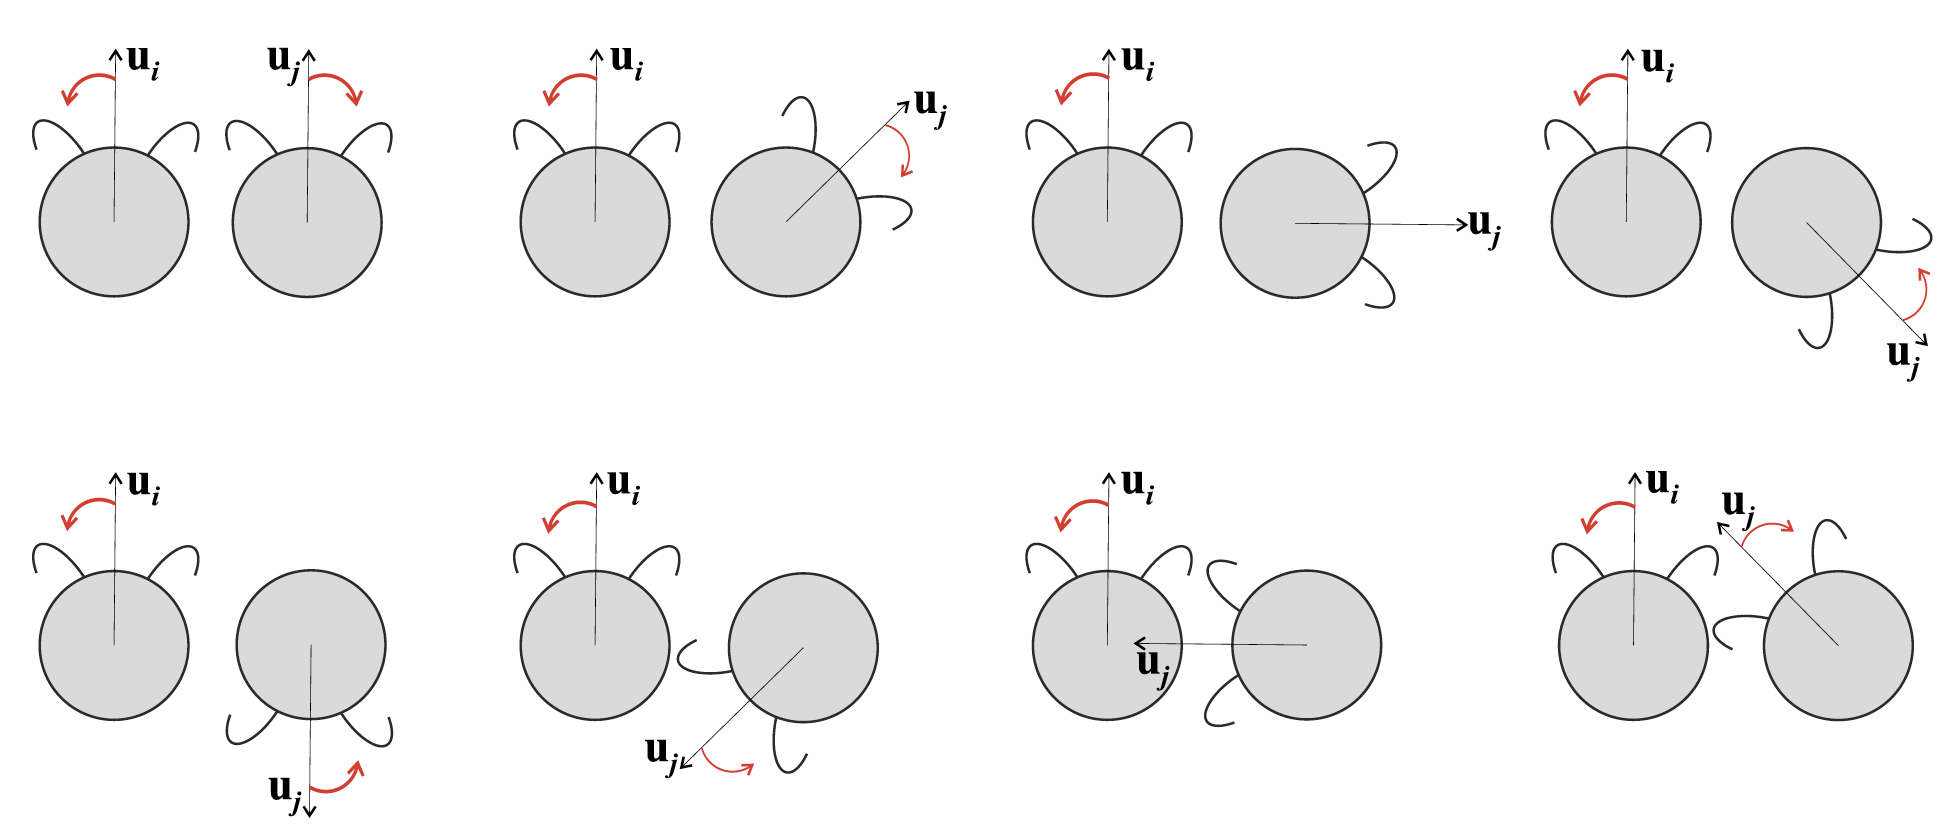
\includegraphics[width=0.9\textwidth]{../images/stark_behavior.png}
        \cite{Stark}
    \end{center}
\end{frame}

\begin{frame}{Numerical Experiments}
    \begin{center}
        Simulation consistent with previous study \cite{Stark}
        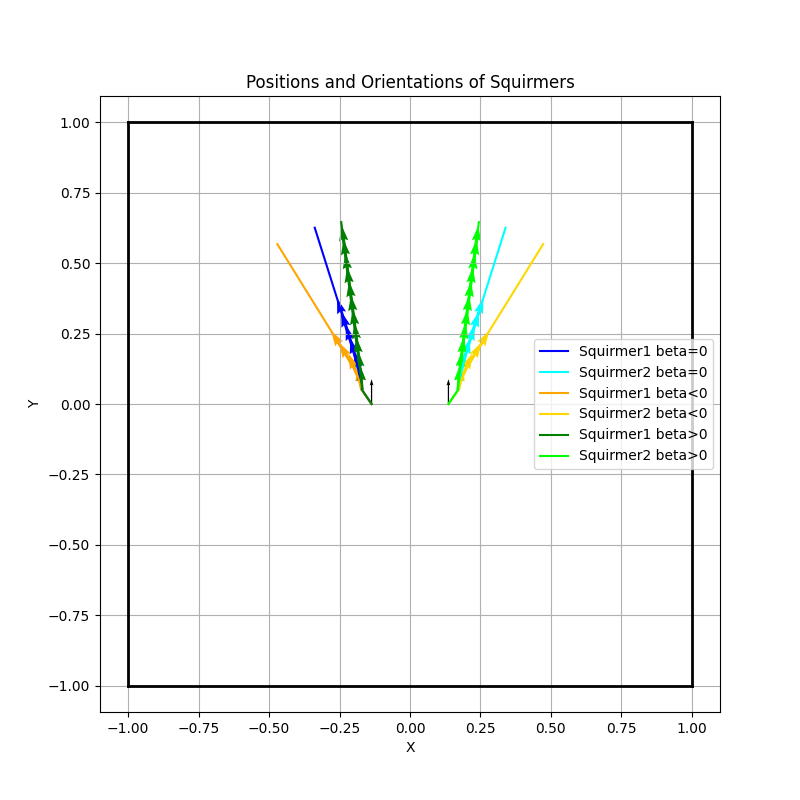
\includegraphics[width=0.8\textwidth]{../../graphs/simulations/twosquirmerinter/sq2.pi.2.png}
    \end{center}
\end{frame}

\begin{frame}{Numerical Experiments}
    \begin{center}
        Example of divergence in results
        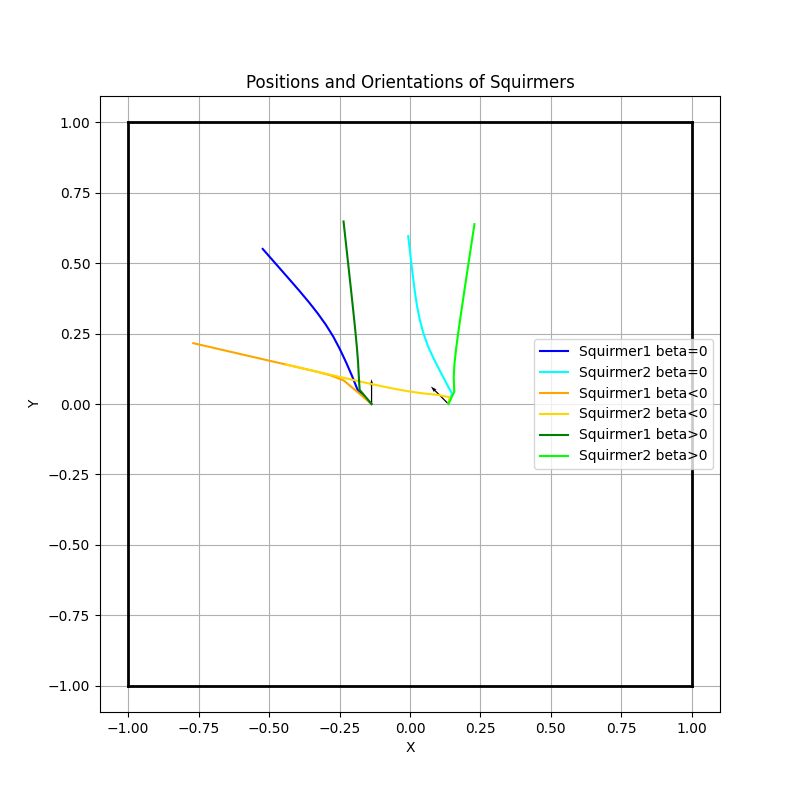
\includegraphics[width=0.8\textwidth]{../../graphs/simulations/twosquirmerinter/sq2.3pi.4.png}
    \end{center}
\end{frame}

\begin{frame}{Numerical Experiments}
    \begin{center}
        Example of divergence in results
        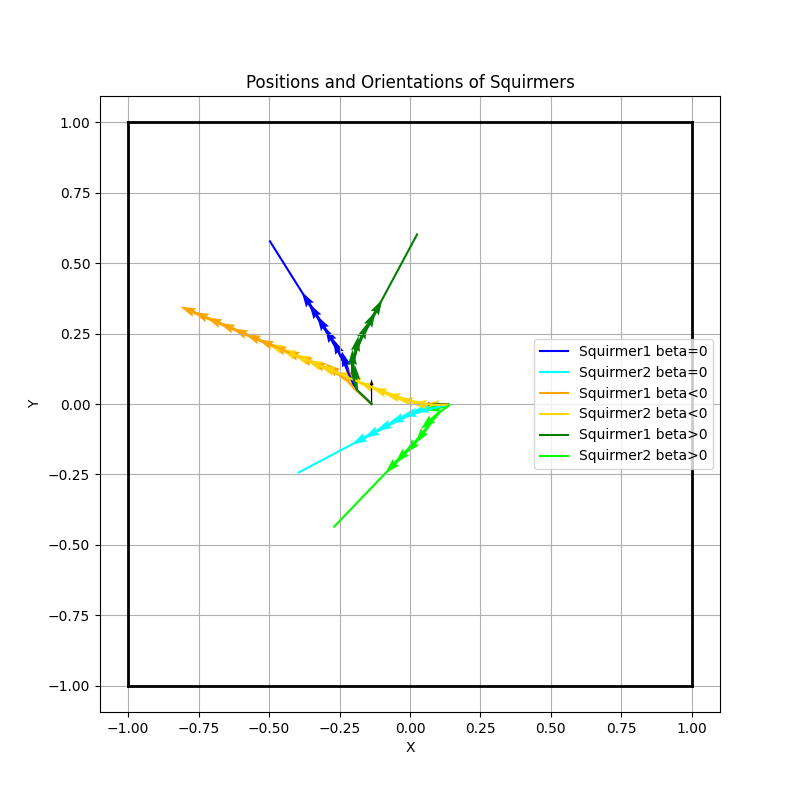
\includegraphics[width=0.8\textwidth]{../../graphs/simulations/twosquirmerinter/sq2.pi.png}
    \end{center}
\end{frame}

\begin{frame}{Conclusion}
    \begin{center}
        \begin{itemize}
            \item Varying $\beta$ value affect behavior
            \item Convergence of results with $\beta = 0$
            \item Discrepancy of results for $\beta \ne 0$
        \end{itemize}
    \end{center}
\end{frame}

\section{References}
\begin{frame}{References}
    \begin{thebibliography}{}
        \bibitem{Brumley} D.R. Brumley and T.J. Pedley, \emph{Stability of arrays of bottom-heavy spherical squirmers}, American Physical Society, 2019
        \bibitem{Lauga} Théry A., Maaß C.C. and Lauga E., \emph{Hydrodynamic interactions between squirmers near walls: far-field dynamics and near-field cluster stability}, Royal Society Open Science, 2023
        \bibitem{Stark} Miloš Knežević,Till Welker \& Holger Stark, \emph{Collective motion of active particles exhibiting non-reciprocal orientational interactions}, Scientific Reports, 2022
        \bibitem{Wikipedia} Wikipédia, \emph{Squirmer}, Wikipédia, 2022
    \end{thebibliography}
\end{frame}

\end{document}